\documentclass[11pt,border=2pt]{standalone}
\usepackage{amsmath,amssymb}
\usepackage{xcolor}
\usepackage{tikz}
\usepackage{pgfplots}
\pgfplotsset{compat=1.18}
\usetikzlibrary{calc,arrows,positioning,fit,backgrounds,decorations.pathreplacing,patterns}
\definecolor{cElem}{RGB}{40,80,140}
\definecolor{cTrg}{RGB}{190,40,40}
\definecolor{cCell}{RGB}{225,238,248}
\definecolor{cAcc}{RGB}{240,200,120}
\definecolor{cGrey}{RGB}{120,120,120}
\definecolor{cVec}{RGB}{110,55,150}
\begin{document}
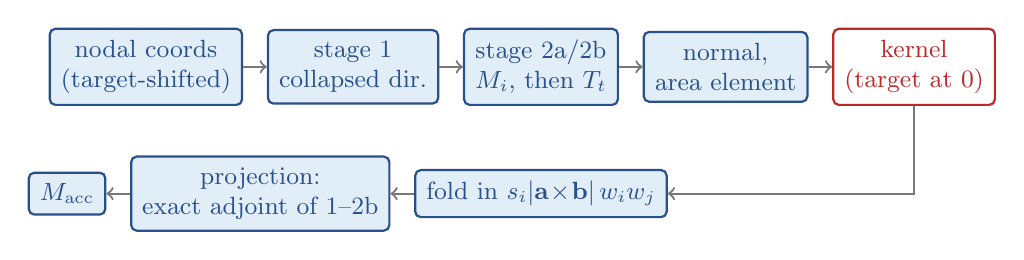
\begin{tikzpicture}[node distance=3mm,
   b/.style={draw,cElem,thick,fill=cCell,rounded corners=2pt,align=center,inner sep=4pt,font=\small},
   k/.style={draw,cTrg,thick,fill=white,rounded corners=2pt,align=center,inner sep=4pt,font=\small},
   a/.style={->,thick,cGrey}]
  \node[b] (f)  {nodal coords\\ (target-shifted)};
  \node[b,right=of f]  (s1) {stage 1\\ collapsed dir.};
  \node[b,right=of s1] (s2) {stage 2a/2b\\ $M_i$, then $T_t$};
  \node[b,right=of s2] (g)  {normal,\\ area element};
  \node[k,right=of g]  (kk) {kernel\\ (target at $0$)};
  \draw[a] (f)--(s1); \draw[a] (s1)--(s2); \draw[a] (s2)--(g); \draw[a] (g)--(kk);
  \node[b,below=8mm of s2] (w) {fold in $s_i|\mathbf{a}\!\times\!\mathbf{b}|\,w_i w_j$};
  \node[b,left=of w] (p) {projection:\\ exact adjoint of 1--2b};
  \node[b,left=of p] (m) {$M_{\text{acc}}$};
  \draw[a] (kk) |- (w); \draw[a] (w)--(p); \draw[a] (p)--(m);
\end{tikzpicture}
\end{document}
